\documentclass[border=0.2cm]{standalone}

% Required packages and libraries
\usepackage{circuitikz}
\usetikzlibrary{calc}

\begin{document}
	
	
	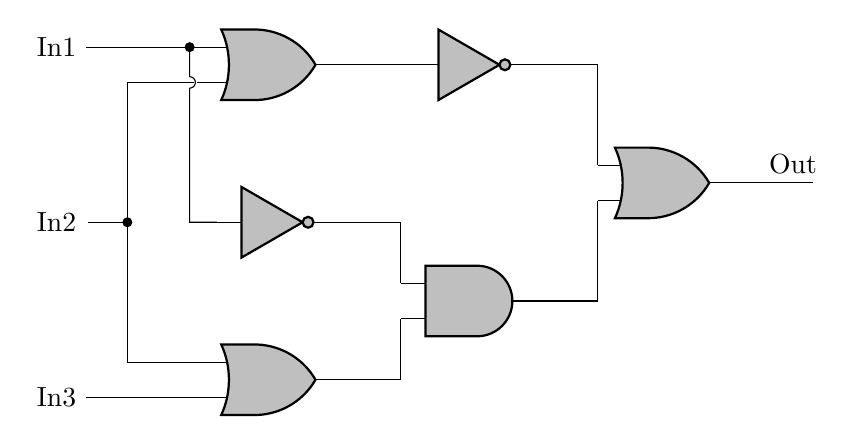
\begin{tikzpicture}
		
		% Circuit style
		\ctikzset{
			logic ports=ieee,
			logic ports/scale=0.8,
			logic ports/fill=lightgray
		}
		
		% Logic ports
		\node[or port] (ORa) at (0,0){};
		\node[not port] (Noa) at (0,-2){};
		\node[or port] (ORb) at (0,-4){};
		
		\node[not port] (Nob) at (2.5,0){};
		\node[and port] (ANDa) at (2.5,-3){};
		
		\node[or port] (ORc) at (5,-1.5){};
		
		% Connection
		\draw (ORa.out) -- (Nob.in);
		
		\draw (Noa.out) -| (ANDa.in 1);
		\draw (ORb.out) -| (ANDa.in 2);
		
		\draw (ANDa.out) -|  (ORc.in 2);
		\draw (Nob.out) -| (ORc.in 1);
		\draw (ORc.out) -- ++(1,0) node[near end,above]{Out};
		
		\draw (ORa.in 1) -- ++(-1.5,0)node[left](In1){In1};
		\draw (ORb.in 2) -- ++(-1.5,0)node[left](In3){In3};
		
		% Jump crossing element
		\node at (ORa.in 2)
		[
		below,
		jump crossing,
		rotate=-90,
		scale=1.3
		](X){};
		
		\draw (Noa.in) -| (X.east)
		(X.west) to[short,-*] (X.west |- ORa.in 1); 
		
		\draw ($ (In1) !.5! (In3) $) node[]{In2}
		++ (0.4,0) to[short,-*] ++(0.5,0) coordinate(a)
		|- (X.south) (a) |- (ORb.in 1);
	\end{tikzpicture}
	
	
\end{document}